\documentclass[11pt]{article}

\usepackage{graphicx}
\usepackage{hyperref}
\usepackage{amsmath, amsthm, amssymb}
\usepackage[toc,page]{appendix}

\author{Phan-Anh Nguyen\\
		286049} 
		
\title{Geometry Processing Lab 2012\\
	   Anisotropic Filtering of Non-Linear Surface Features}
	   
\begin{document}
\maketitle



\section{Introduction}

Nowadays, geometric data acquired through imaging or scanning devices has grown rapidly due to advances in technology, making it affordable in many aspects of our lives. However, when dealing with real data we always have to cope with measurement error which brings high frequency noise to our geometric models. Many researches have been conducted in order to remove noise from a scanned model while trying to preserve the underlying sampled surface. One of the seminal results was the work of Taubin et al. \cite{Taubin:1995:SPA:218380.218473} in which they use a signal processing approach to derive the Laplacian operator acting as a low-pass filter on the geometric signal. Even though the Laplacian operator is a powerful tool to remove high frequency noise, it isotropic behaviour makes it unable to preserve sharp features. Hildebrandt and Polthier \cite{Hildebrandt04anisotropicfiltering} have developed an anisotropic method which can preserve high curvature features in a certain direction while suppressing unwanted curvature peaks in the other directions. This method makes it possible to denoise arbitrary surface meshes whereas non-linear geometric features e.g. curved surface regions and feature lines are preserved. This lab report explores and elaborates theory and practice needed to implement the prescribed mean curvature flow proposed by Hildebrandt and Polthier \cite{Hildebrandt04anisotropicfiltering}.

\section{Smoothing Principle}

\begin{figure}[htbp]
  \begin{minipage}[b]{0.45\linewidth}
    \centering
    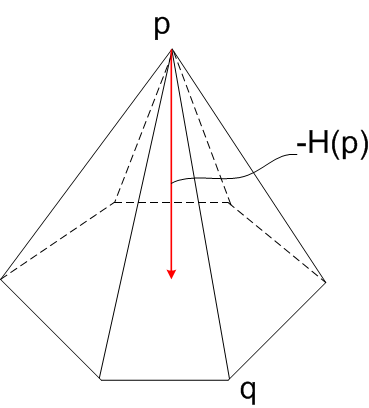
\includegraphics[width=\textwidth]{umbrella.png}
    \caption{smooth a vertex p by moving it in the direction of the mean curvature vector $\vec{H}(p)$}
    \label{fig:umbrella}
  \end{minipage}
  \hspace{0.5cm}
  \begin{minipage}[b]{0.45\linewidth}
    \centering
    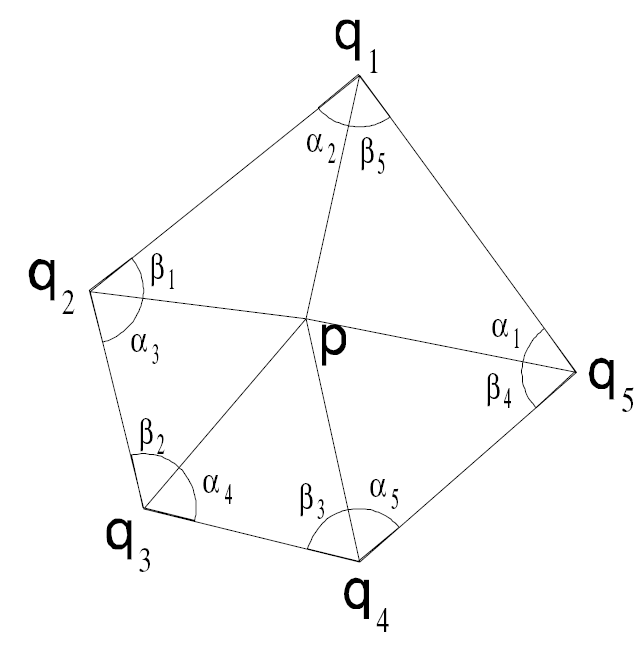
\includegraphics[width=\linewidth]{cotangent.png}
    \caption{Cotangent weights}
    \label{fig:cotangent}
  \end{minipage}
\end{figure}

A very intuitive smoothing operator one can think of is to move a vertex $p$ to the center of gravity (c.o.g) of its one-ring neighbors $N_1(p)$:

\begin{equation}
p \leftarrow \frac{1}{\mid N_1(p) \mid}\sum\limits_{q \in N_1(p)}q = p - \underbrace{\frac{1}{\mid N_1(p) \mid}\sum\limits_{q \in N_1(p)}(p - q)}_{\bigtriangleup p}
\label{eq:update}
\end{equation}

Equation $\ref{eq:update}$ reveals the update form of the smoothing operator in which the old vertex is moved by an amount of the update vector $\bigtriangleup p$ to the new position. The update vector $\bigtriangleup p$ can be generalized to have arbitrary weights over the 1-ring $\sum\limits_{q \in N_1(p)}w_q(p - q)$ other than uniform weights as in the equation $\ref{eq:update}$. In fact, we can choose the weights such that the update vector points in the direction normal to the mesh surface. Such an update formula was first proposed by Pinkall and Polthier \cite{Pinkall93computingdiscrete} known as cotangent weights:

\begin{equation}
\bigtriangledown_p\ area = \vec{H}(p) = 1/2\sum\limits_{q \in N_1(p)}{(cot\alpha_{q} + cot\beta_{q})(p-q)}
\label{eq:cotangent}
\end{equation}

Where $\vec{H}(p)$ is the mean curvature vector at a vertex $p$ and equal the gradient of the area functional $\bigtriangledown_p\ area$ at that vertex. Figure $\ref{fig:umbrella}$ and $\ref{fig:cotangent}$ show how the mean curvature vector is calculated.

\section{Anisotropic Mean Curvature}

The first step towards deriving an anisotropic mean curvature formula is to express the vertex mean curvature vector $\ref{eq:cotangent}$ in terms of an edge based mean curvature vector:
\begin{equation}
  \vec{H}(e) = H_e \vec{N}_e
  \label{eq:edgeMC}
\end{equation}
where $N_e = \frac{N_1 + N_2}{\parallel N_1 + N_2 \parallel}$ is the edge normal vector as shown in figure $\ref{fig:curvature}$ and $H_e = 2\mid e \mid \cos \frac{\theta_e}{2}$ is the edge mean curvature which depends on the dihedral angle $\theta_e$ as illustrated in figure $\ref{fig:dihedral}$. Note that the smaller the dihedral angle, the sharper the edge thus resulting in the higher the mean curvature $H_e$. Therefore, the term $H_e$ can be seen as the measurement of the directional curvature of the surface in the direction orthogonal to the edge.

\begin{figure}[htbp]
  \begin{minipage}[b]{0.45\linewidth}
	\centering
	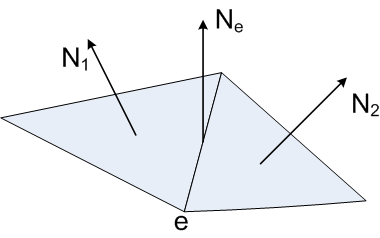
\includegraphics[width=\textwidth]{curvature.png}
	\caption{Edge normal vector $N_e$}
	\label{fig:curvature}
  \end{minipage}
  \hspace{0.5cm}
  \begin{minipage}[b]{0.45\linewidth}
    \centering
    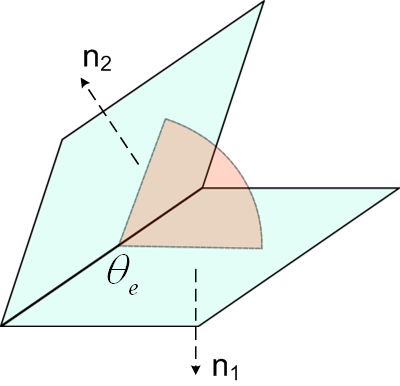
\includegraphics[width=\linewidth]{dihedral.png}
    \caption{Dihedral angle $\theta_e$}
    \label{fig:dihedral}
  \end{minipage}
\end{figure}

It can be shown, in the work of Polthier \cite{PolthierHabilitation}, that the vertex mean curvature vector $\vec{H}(p)$ and the edge mean curvature vector $\vec{H}(e)$ are related by the equation:

\begin{equation}
\vec{H}(p) = \frac{1}{2}\sum\limits_{e = (p, q), q \in N_1(p)}\vec{H}(e)
\end{equation}

The anisotropic mean curvature vector $\vec{H}_A$ at a vertex $p$ is then defined as a weighted sum over the contributions $H_e\vec{N}_e$ at the edges incident to a vertex $p$:

\begin{equation}
\vec{H_A}(p) = 1/2\sum\limits_{e = (p, q), q \in N_1(p)}{w(H_e)H_e \vec{N}(e)}
\label{eq:aniso}
\end{equation}

The weight function $w$ is used to put less weight on feature vertices in order to avoid smoothing sharp features:

\begin{equation}
w_{\lambda, r}(a) = 
\begin{cases}
1 & \text{for } |a| \leq \lambda \\
\dfrac{\lambda^2}{r(\lambda - |a|)^2+\lambda^2} & \text{for } |a| > \lambda
\end{cases}
\end{equation}

The threshold $\lambda$ is used to detect features and the radius $r$ controls the width of the transition between those areas that are smoothed and those that are kept as features. In our implementation, we choose $\lambda = 2 \lambda' \max |e| $ where $\lambda' \in \left[ 0, 1 \right] $ to cover the whole range of the edge mean curvature $H_e$. Following Hildebrandt and Polthier suggestion \cite{Hildebrandt04anisotropicfiltering}, we fix the radius $r$ to 10 to ensure that $w_{\lambda, 10}(2\lambda) < 0.1$.

The smoothing operation is carried out by integrating the flow of the anisotropic mean curvature vector $\vec{H}_A$ with some integration scheme. We first use the explicit Euler method because it is simpler to implement. Discussion about the semi-implicit integration scheme will be presented later on.

Given the mesh $M_h$ with its vertices $\mathcal{P} = \left\lbrace p_1, ..., p_m \right\rbrace $, an explicit iteration step of the anisotropic mean curvature flow is computed as follows:

\begin{equation}
\mathcal{P}^{j+1} = \mathcal{P}^j -sM^{-1}\vec{H_A}(\mathcal{P}^j)
\label{eq:explicit}
\end{equation}

where $s \in [0, 1]$ is a damping factor controlling the magnitude of the update vector thereby stabilizing the flow. $M^{-1}$ is the inverse of the mass matrix $M \in \mathcal{R}^{m \times m}$ of the mesh $M^j_h$ at time step $j$. It is used to convert the integrated mean curvature vector into a piecewise linear vector field:

\begin{equation}
M_{pq} = 
\begin{cases} \dfrac{1}{6}area(star\ p), & \mbox{if } p=q \\ 
\dfrac{1}{12}area(star\ e), & \mbox{if there is an edge } e=(p, q) \\
0, & \mbox{otherwise} \end{cases}
\label{eq:mass_matrix}
\end{equation}

If we use a diagonalization of $M$ called the lumped mass matrix with diagonal elements $M_{pp} = \frac{1}{3} area(star\ p)$, then the integration step for each vertex $p$ is derived as follows:

\begin{equation}
p^{j+1} = p^{j} - \dfrac{3s}{area(star\ p^j)}\vec{H_A}(p^j)
\end{equation}

One disadvantage of the lumped mass matrix is that it gives an unstable solution. To overcome this problem we have to use a very small time step leading to a slow convergence rate. In contrast, the full mass matrix gives a more stable solution, thereby giving a faster convergence rate with the cost of having to compute the inverted mass matrix.

\section{Prescribed Mean Curvature}

Since the mean curvature vector at a vertex is equivalent to its area gradient, applying the mean curvature flow on the mesh has the same effect as minimizing its surface area. This leads to the problem of surface shrinkage. This issue also occurs in the anisotropic case. Particularly, the anisotropic smoothing slows down the smoothing process in regions with high curvature, causing
deformations of the surface as shown in figure $\ref{fig:amc_pmc}$.

\begin{figure}[htb]
\centering
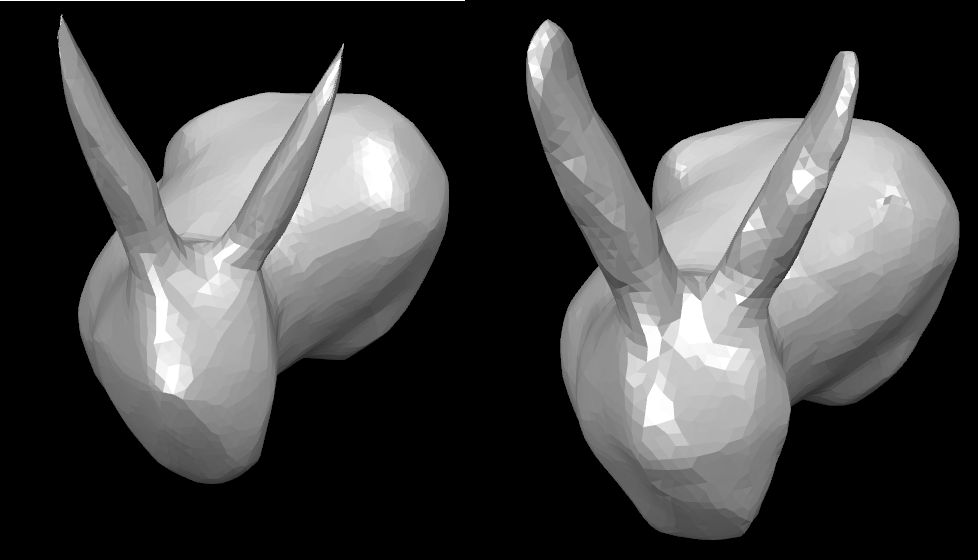
\includegraphics[width=\textwidth]{amc_pmc.png}
\caption{The Anisotropic Mean Curvature flow (left) contracts the interior of the bunny's ears making it to deform. In contrast, the Prescribed Mean Curvature flow (right) converges to a stable surface.}
\label{fig:amc_pmc}
\end{figure}

To circumvent this problem, Hildebrandt and Polthier \cite{Hildebrandt04anisotropicfiltering} used the so-called prescribed mean curvature flow (PMC) to evolve the surface towards a surface having a prescribed mean curvature. This process includes two steps. In the first step, the surface mean curvature is computed and then this scalar field is smoothed. In the second step, the PMC flow is applied to let the surface evolve towards a surface with this precomputed mean curvature. 

This idea comes from the result \cite{PolthierRossmann2002} given as follows:

\begin{equation}
\vec{H_A}(p) = \bigtriangledown_p area = H \bigtriangledown_p vol
\label{eq:evolution}
\end{equation}

for all interior vertices $p$ and a constant mean curvature $H$. Hence instead of minimizing the anisotropic mean curvature vector $\vec{H_A}(p) \rightarrow 0$, we let $\vec{H_A}(p)$ evolve to the prescribed mean curvature according to equation $\ref{eq:evolution}$, i.e. $\vec{H_A}(p) \rightarrow H\vec{V_A}(p)$. The anisotropic PMC flow thus is defined by:

\begin{equation}
\mathcal{P}^{j+1} = \mathcal{P}^j -sM^{-1}(\vec{H_A}(\mathcal{P}^j) - f(\mathcal{P}) \cdot \vec{V}_A(\mathcal{P}))
\label{eq:pmc}
\end{equation}

where $f$ is a function that prescribes the anisotropic mean curvature and $\vec{V}_A$ is an anisotropic volume gradient. The volume of a surface is the oriented volume enclosed by the cone of the surface over the origin in $\mathcal{R}^3$:

\begin{equation}
vol \ M_h = \sum\limits_{T=(p, q, r) \in M_h}vol(tetrahedron(o, p, q, r)) = \frac{1}{6}\sum\limits_{T=(p, q, r) \in M_h}<p, q \times r>
\label{eq:volume}
\end{equation}

Figure $\ref{fig:volume}$ illustrates how the volume of a surface is calculated. Note that the volume of tetrahedrons is negative in front-facing regions (where the normal pointing to the origin). This negative volume cancels out with the volume of back-facing tetrahedrons hence only the volume enclosed by the surface is computed.

\begin{figure}[htbp]
  \begin{minipage}[b]{0.45\linewidth}
\centering
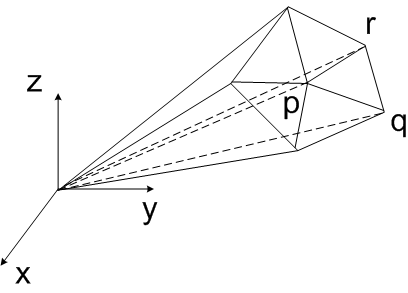
\includegraphics[width=\textwidth]{volume.png}
\caption{volume of a surface is the sum of volume of oriented tetrahedrons spanned by surface triangles with the origin.}
\label{fig:volume}
  \end{minipage}
  \hspace{0.5cm}
  \begin{minipage}[b]{0.45\linewidth}
\centering
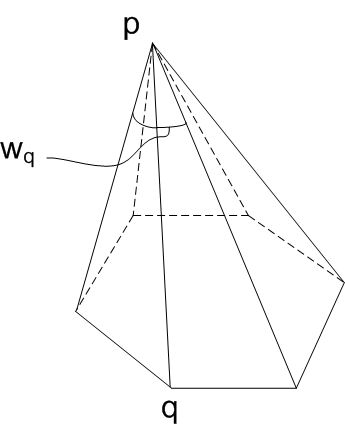
\includegraphics[width=\textwidth]{vertex_angles.png}
\caption{sum of vertex angles $\omega_q$.}
\label{fig:vertex_angle}
  \end{minipage}
\end{figure}

Since $vol \ M_h$ linearly depends on $p$, the gradient of $vol \ M_h$ at $p$ is easily derived from $\ref{eq:volume}$ as follows:

\begin{equation}
\bigtriangledown_p vol = \frac{1}{6}\sum\limits_{T=(p, q, r) \in M_h}q \times r
\end{equation}

Having defined the volume gradient we can now derive its anisotropic counterpart $\vec{V}_A$ as introduced in equation $\ref{eq:pmc}$. For non-feature vertices $p$, i.e. $\vec{H}_A(p) = \vec{H}(p)$, $\vec{V}_A(p)$ is set to $\bigtriangledown_p(vol)$. For the other vertices $\vec{V}_A(p)$ is defined by:

\begin{equation}
\vec{V}_A(p) = sign\left( \left\langle \vec{e}_{H_A}(p), \bigtriangledown_p vol\right\rangle \right) \vec{e}_{H_A}(p)
\end{equation}

where $\vec{e}_{H_A}(p)$ is the unit vector field of $\vec{H}^s_A$ and we get $\vec{H}^s_A$ by performing a simple smoothing step on $\vec{H}_A$:

\begin{equation}
\vec{H}^s_A(p) = \frac{1}{2}\left( \vec{H}_A(p) + \dfrac{1}{\sum\limits_{q \in N_1(p)} \omega_q}\sum\limits_{q \in N_1(p)}\omega_q\vec{H}_A(q) \right) 
\end{equation}

\begin{equation}
\vec{e}_{H_A}(p) = \dfrac{\vec{H}^s_A(p)}{\parallel \vec{H}^s_A(p) \parallel}
\end{equation}

where $\omega_q$ is the sum of the vertex angles at $p$ in the triangles adjacent to the edge $\bar{pq}$ as displayed in figure $\ref{fig:vertex_angle}$.

The function $f$ is computed according to the formula $f = M^{-1}H_A$. To avoid computing the inverse of the mass matrix in each step Hildebrandt and Polthier \cite{Hildebrandt04anisotropicfiltering} approximate $f$ by $H_A(p)/\parallel \vec{V}_A(p) \parallel$. After that the scalar field prescribed by $f$ at each vertex $p$ is smoothed by averaging over neighbor vertices of $p$. To preserve sharp edges, each feature vertex $p$ is only averaged over those neighbor vertices that are feature vertices as well. Finally the update formula for each vertex $p$ utilizing the lumped mass matrix is given in the following:

\begin{equation}
p^{j+1} = p^{j} - \dfrac{3s}{area(star\ p^j)}(\vec{H_A}(p^j) - f(p^j)\vec{V_A}(p^j))
\end{equation}

\section{Implementation and Results}

For the implementation, we use OpenFlipper framework \cite{springerlink:10.1007} which supports Mesh manipulation, Graphical User Interface and many utilities including OpenMesh \cite{Botsch02openmesh-} for Halfedge data structure. We use Eigen library \cite{eigenweb} and CHOLMOD \cite{Davis:2009:DSS:1462173.1462176} for matrix operations.

For testing purpose, we develop an adaptive noise generator which generate noisy model based on local edge length while avoiding folded mesh. We also use color coding with the color range from zero to the maximum difference between a vertex from the true model and a vertex from the smoothed model.

In figure $\ref{fig:amc_pmc}$ we have already seen the effect of applying anisotropic mean curvature flow versus the prescribed mean curvature flow. In this configuration, we use the lumped mass matrix and use a very small time step of 0.000001 with 100 iterations. Note that the time step depends on the edge length, so with the larger model we could expect the larger time step. obviously in this case, PMC flow gives better result.

Figure $\ref{fig:results}$ compares the results of applying the full mass matrix as against the lumped mass matrix. The figure on the left shows PMC flow with lumped mass matrix after 200 iterations. In this case, we use a small time step at 0.00001 and set the feature detector $\lambda = 0.5$. The result still shows some noise on the top of the model but there is some sign of over smoothed on the fading ridge. The figure in the middle shows PMC flow with full mass matrix after 100 iterations. This time we use a larger time step at 0.001 and use a smaller feature detector value $\lambda = 0.3$ making it more sensitive to features. The result shows that, not only can we keep the sharp feature at the fading ridge, we can still get rid of the noise on the top of the model. Unfortunately, we have to invert the mass matrix for each iteration, thereby making it much slower than using the lumped mass matrix. The color coding additionally shows the good convergence to the ground truth.

\begin{figure}[htb]
\centering
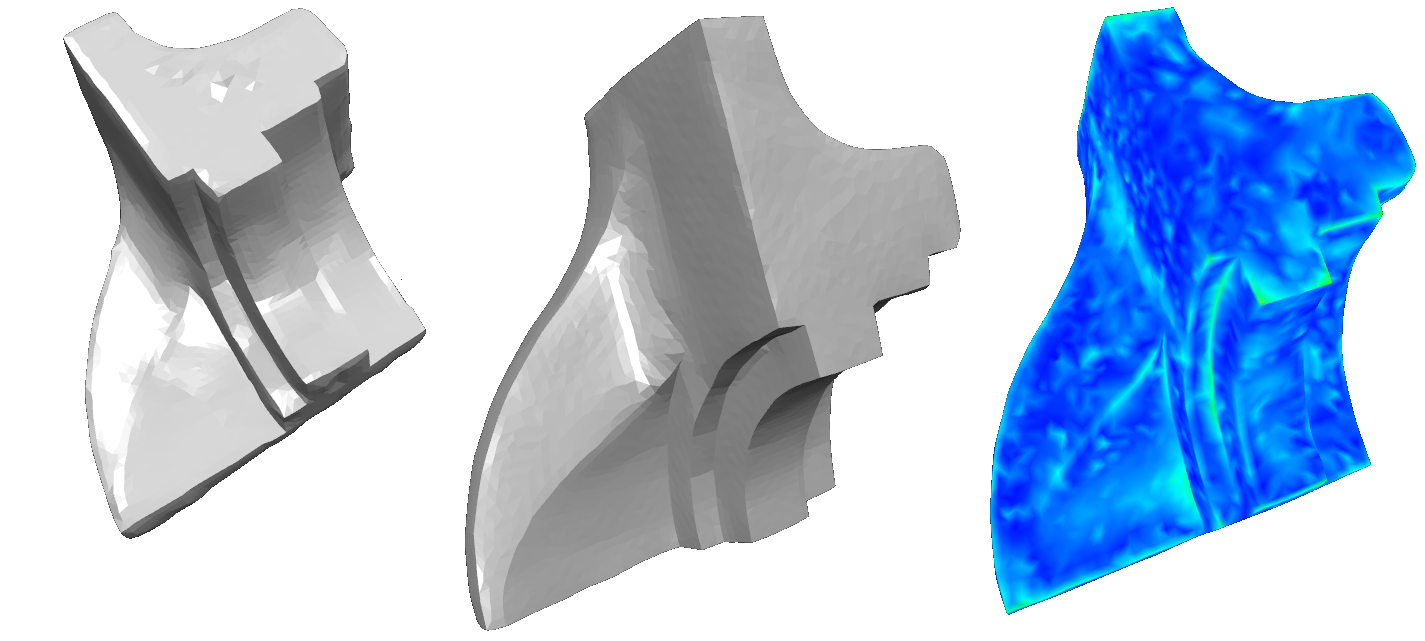
\includegraphics[width=\textwidth]{results.png}
\caption{From left to right: PMC flow with lumped mass matrix, PMC flow with full mass matrix, Color coding for PMC flow with full mass matrix.}
\label{fig:results}
\end{figure}

Finally, figure $\ref{fig:compare}$ compares the results from the squared Laplacian smoothing operator and the PMC flow. Since the squared Laplacian treats the curvature equally in all directions, it cannot preserve sharp edges. In contrast, the PMC flow can detect features based on the directional measurement of curvature, hence it can avoid smoothing in high curvature regions.

\begin{figure}[htb]
\centering
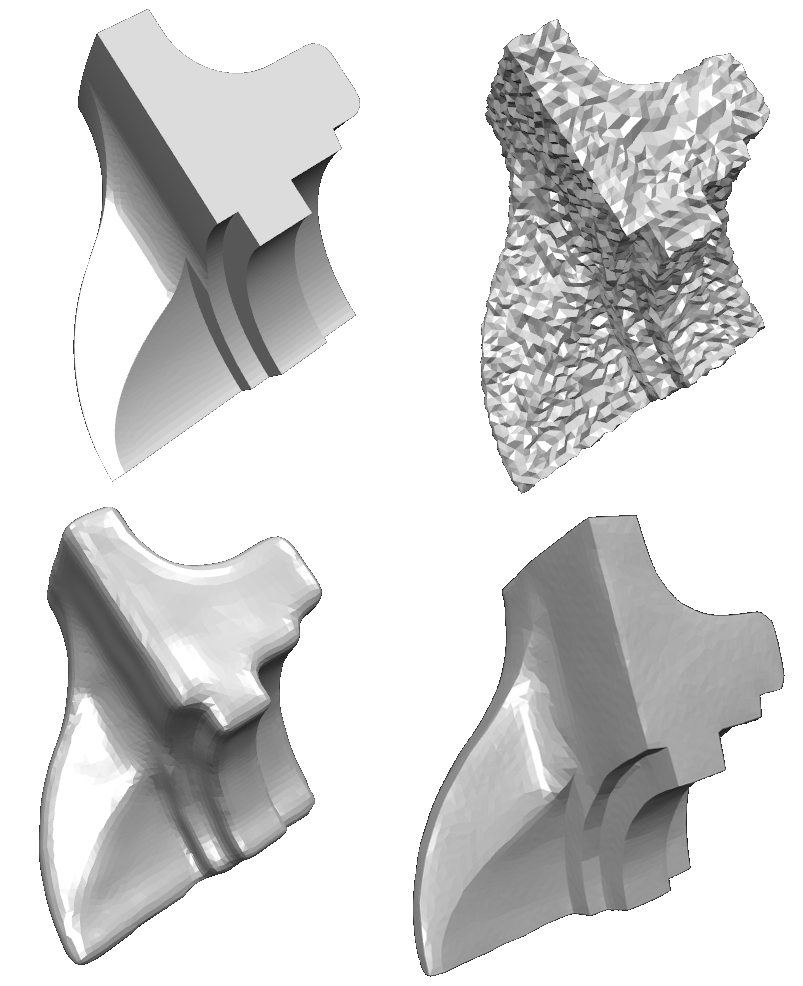
\includegraphics[width=\textwidth]{amc_laplacian.png}
\caption{Top left: original model, top right: noisy model, bottom left: squared Laplacian, bottom right: PMC flow.}
\label{fig:compare}
\end{figure}

\section{Conclusion and Future Work}

This report focused on evaluating the anisotropic filtering methods developed by Hildebrandt and Polthier \cite{Hildebrandt04anisotropicfiltering}. The authors decomposed the vertex-based mean curvature into the sum of the edge-based mean curvature in the neighborhood of the vertex. The edge-based mean curvature measures the directional curvature connected to that edge leading to the definition of the anisotropic mean curvature vector. Besides the anisotropic mean curvature flow, they also proposed the prescribed mean curvature flow to let the surface evolve to a surface with prescribed mean curvature. This report explored the explicit integration scheme for both two kind of flows. The appendix $\ref{apx:implicit}$ will discuss some attempts to deal with the implicit integration method which is also open for future work.

\bibliographystyle{alpha}
\bibliography{bibliography}

\begin{appendices}
\section{Attempts towards semi-implicit Integration}
\label{apx:implicit}

The idea of a semi-implicit scheme is to shift part of the calculation to the current time step instead of computing the update based entirely on the previous time step. In order to apply this idea into our problem, we start from the explicit integration scheme in equation $\ref{eq:explicit}$

\end{appendices}

\end{document}